%% Relatorio de progresso PPC baseado no template oficial preliminary/template.tex.
\documentclass[sigplan]{acmart}
\settopmatter{printacmref=false}
\renewcommand\footnotetextcopyrightpermission[1]{}
\usepackage{array}
\usepackage{graphicx}
\usepackage{tikz}
\usetikzlibrary{arrows.meta,positioning}
\usepackage{booktabs}

\begin{document}

\title{Modelos de Concorrência num Microserviço Java: Resultados Preliminares}

\author{Pedro Gomes}
\affiliation{%
 \institution{Programação Paralela e Concorrente\\
  Mestrado em Engenharia Informática\\
  Faculdade de Ciências, Universidade de Lisboa}
 \city{Lisboa}
 \country{Portugal}}
\email{fc67991@alunos.ciencias.ulisboa.pt}

\begin{abstract}
Este relatório apresenta resultados preliminares da comparação entre platform threads, virtual threads e I/O assíncrono num agregador Spring Boot que chama um serviço HTTP simulado (RQ1 da proposta). Num piloto com k6 a 10, 100 e 500 utilizadores virtuais (VUs), os três modelos tiveram desempenho próximo até 100 VUs. A 500 VUs, virtual e async atingiram cerca de 404 pedidos/s com p99 de 1,13 s, contra 184 pedidos/s e p99 de 2,84 s nas platform threads, um padrão consistente com a hipótese H1. Com uma medição por condição e na mesma máquina, os resultados são exploratórios e não permitem conclusões gerais.
\end{abstract}

\pagestyle{plain}
\maketitle

\section{Contexto e questões de investigação}
Os microserviços passam grande parte do tempo à espera de respostas externas, pelo que o modelo de concorrência condiciona o seu desempenho sob carga. A proposta define duas questões e hipóteses:

\noindent\textbf{RQ1.} Como variam o throughput e a latência dos três modelos com o aumento dos pedidos concorrentes?
\textbf{H1.} Sob concorrência elevada e carga I/O-bound, virtual threads e I/O assíncrono superam platform threads em throughput e latência de cauda.

\noindent\textbf{RQ2.} Como influenciam a latência externa, chamadas por pedido e trabalho de CPU o desempenho relativo dos modelos?
\textbf{H2.} As vantagens de virtual threads e async diminuem com o aumento de trabalho de CPU. Este relatório cobre o piloto da RQ1; a RQ2 é o trabalho seguinte.

\section{Arquitetura e implementação}
O protótipo tem um agregador Spring Boot (porta 8081) e um stub (porta 8080) que aguarda 1\,000~ms e devolve JSON. O stub usa \texttt{spring.threads.virtual.enabled=true} para evitar que o serviço simulado limite a carga.

\begin{figure}[t]
\centering
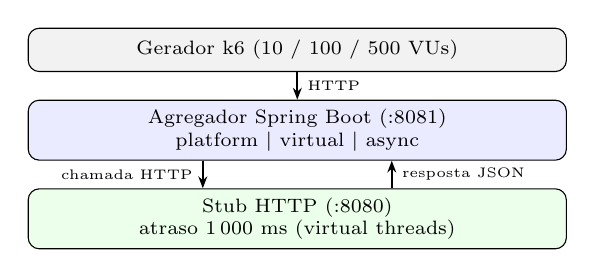
\begin{tikzpicture}[font=\scriptsize,
 box/.style={draw,rounded corners,align=center,minimum height=5.5mm,text width=66mm},
 arr/.style={-{Stealth[length=1.5mm]},thick}]
\node[box,fill=gray!10] (load) {Gerador k6 (10 / 100 / 500 VUs)};
\node[box,below=3.5mm of load,fill=blue!8] (agg) {Agregador Spring Boot (:8081)\\platform \textbar\ virtual \textbar\ async};
\node[box,below=3.5mm of agg,fill=green!8] (stub) {Stub HTTP (:8080)\\atraso 1\,000~ms (virtual threads)};
\draw[arr] (load) -- node[right,font=\tiny]{HTTP} (agg);
\draw[arr] ([xshift=-12mm]agg.south) -- node[left,font=\tiny]{chamada HTTP} ([xshift=-12mm]stub.north);
\draw[arr] ([xshift=12mm]stub.north) -- node[right,font=\tiny]{resposta JSON} ([xshift=12mm]agg.south);
\end{tikzpicture}
\caption{Arquitetura do ensaio. Os três endpoints do agregador fazem uma chamada equivalente ao stub.}
\label{fig:architecture}
\end{figure}

No módulo agregador, implementaram-se os três modelos de concorrência para o mesmo percurso: (i)~com \textbf{platform threads}, a thread do Tomcat bloqueia na chamada externa; (ii)~com \textbf{virtual threads}, o pedido corre numa virtual thread dedicada via \texttt{CompletableFuture}; (iii)~no modelo \textbf{assíncrono}, \texttt{HttpClient.sendAsync()} liberta a thread durante o I/O. O percurso e trabalho funcional são idênticos nos três modos~\cite{jep444}. O código-fonte está disponível em~\cite{repogit}.

\section{Metodologia do piloto}
O k6 executou uma vez cada combinação de modo e concorrência (10, 100 e 500 VUs): subida/aquecimento de 10~s, carga constante de 30~s, descida de 5~s e timeout de 15~s. Foram recolhidos throughput, p50/p95/p99 e erros, usando as métricas incorporadas do k6~\cite{k6metrics}. O ambiente de ensaio foi Windows~10 Home (64-bit), CPU Intel Core i5-10400F (6 núcleos / 12 threads @ 2,90~GHz), 16~GB de RAM DDR4, Eclipse Adoptium Temurin OpenJDK 21.0.13 (LTS) e Maven 3.10.0. Gerador, agregador e stub correram na mesma máquina.

O piloto é um subconjunto deliberado da proposta (Tabela~\ref{tab:scope}): serve para validar a metodologia e reduzir o âmbito antes das medições finais.

\begin{table}[h!]
\caption{Proposta versus piloto.}
\label{tab:scope}
\centering\scriptsize
\renewcommand{\arraystretch}{0.88}
\setlength{\tabcolsep}{3pt}
\begin{tabular}{>{\raggedright\arraybackslash}p{.24\columnwidth}>{\raggedright\arraybackslash}p{.35\columnwidth}>{\raggedright\arraybackslash}p{.32\columnwidth}}
\toprule
Aspeto & Proposta & Piloto\\
\midrule
Concorrência & 10, 100, 1000, 2000 & 10, 100, 500 VUs\\
Latência stub & fixa, variável, cauda & fixa (1\,000 ms)\\
Chamadas & 1, 3, 5 por pedido & 1\\
Carga de CPU & nenhum, moderado, alto & nenhum\\
Métricas & throughput, latência, RAM & throughput, latência\\
Gerador & máquina externa & mesma máquina\\
Repetições & várias com dispersão & uma única execução\\
\bottomrule
\end{tabular}
\end{table}

\section{Resultados}
Até 100 VUs, as três variantes apresentam throughput e latências próximos (Figuras~\ref{fig:throughput} e~\ref{fig:p99}). A 500 VUs (Tabela~\ref{tab:500}), as platform threads ficam perto de 184 pedidos/s e p99 de 2,84~s; virtual e async ficam perto de 404 pedidos/s e p99 de 1,13~s, ou seja, cerca de $2{,}2\times$ o throughput e $2{,}5\times$ menos latência de cauda.
Os nove resultados guardados registam 0\% de erros. Entre virtual e async, as diferenças são inferiores a 3\% em todas as métricas, mas, sem repetições, não é possível saber se são ruído; a proximidade não demonstra equivalência nem superioridade geral.

\begin{figure}[t]
\centering
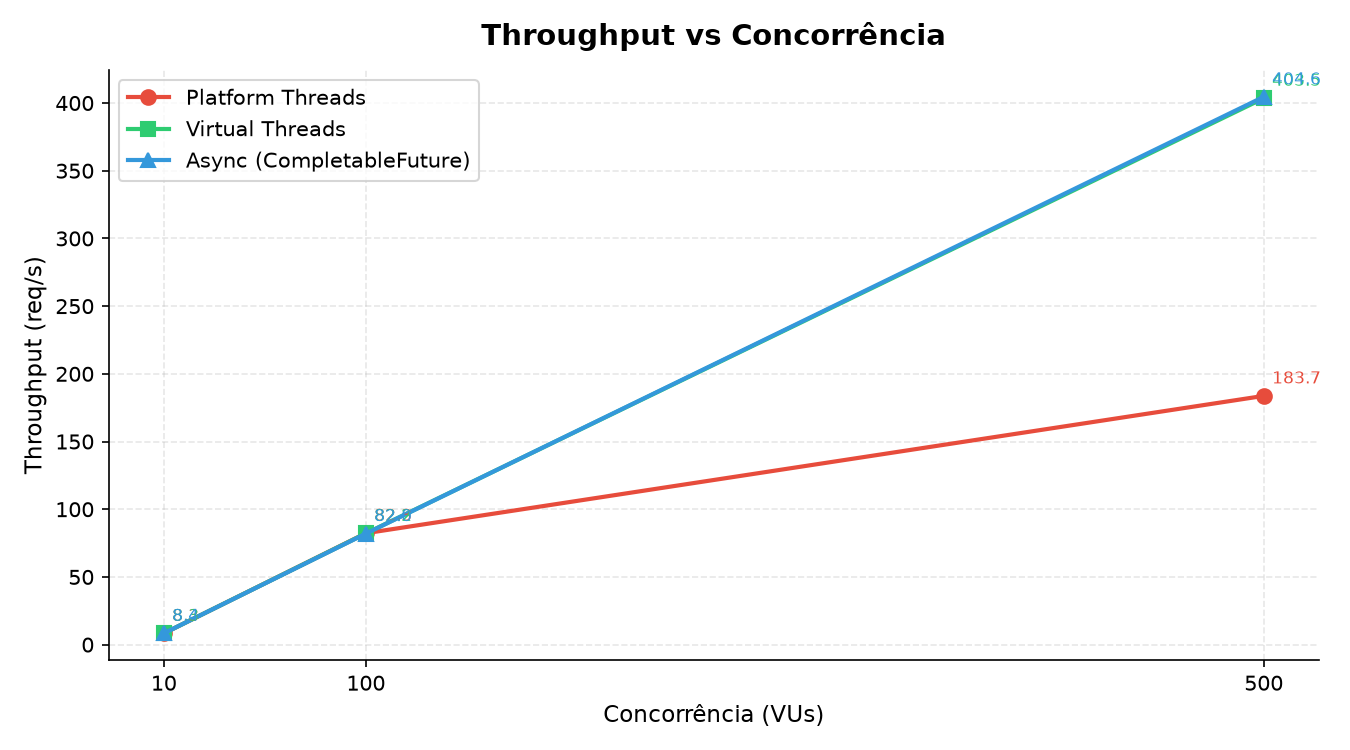
\includegraphics[width=0.82\columnwidth]{../benchmarks/results/figures/throughput_vs_concurrency.png}
\caption{Throughput por concorrência.}
\label{fig:throughput}
\end{figure}

\begin{figure}[t]
\centering
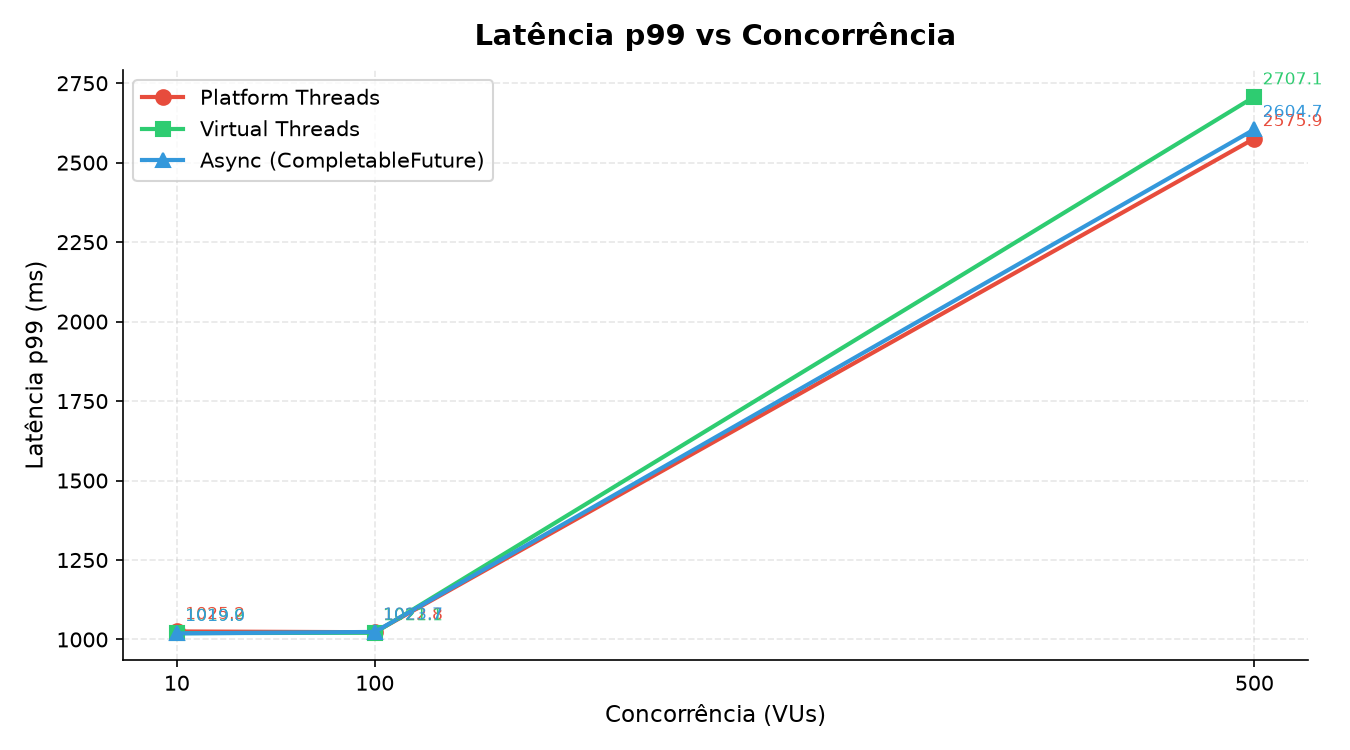
\includegraphics[width=0.82\columnwidth]{../benchmarks/results/figures/latency_p99_vs_concurrency.png}
\caption{Latência p99 por concorrência.}
\label{fig:p99}
\end{figure}

\begin{table}[t]
\caption{Resultados a 500 VUs (uma execução por modo).}
\label{tab:500}
\centering\small
\begin{tabular}{lrrrr}
\toprule
Modo & req/s & p50 (ms) & p95 (ms) & p99 (ms)\\
\midrule
Platform & 183,71 & 2\,477,89 & 2\,793,12 & 2\,837,45\\
Virtual & 403,53 & 1\,018,53 & 1\,091,43 & 1\,133,70\\
Async & 404,58 & 1\,015,83 & 1\,060,21 & 1\,138,17\\
\bottomrule
\end{tabular}
\end{table}

\smallskip\noindent\textbf{Relação com estudos anteriores.} Dundov~\cite{dundov2026} observou que virtual threads em Spring Boot superam platform threads sob carga I/O-bound elevada; Pandita~\cite{pandita2024} reportou ganhos equivalentes em workloads de alto débito com I/O bloqueante. Os resultados deste piloto alinham-se com esses estudos: a vantagem de ${\approx}2{,}2\times$ em throughput e ${\approx}2{,}5\times$ em latência de cauda surge a 500~VUs, quando o pool de platform threads se torna o gargalo. A convergência dos três modelos até 100~VUs é também consistente com a literatura: a diferença de desempenho só se manifesta quando a concorrência pressiona os recursos de threading.

\smallskip\noindent\textbf{Relação com H1.} Os resultados a 500 VUs são consistentes com H1: o modelo bloqueante em platform threads satura e os outros dois não. Mas H1 refere concorrência elevada e a proposta prevê 1000 e 2000 VUs, ainda não testados, e com uma repetição por condição não há estimativa de variabilidade nem teste estatístico. H1 fica, por agora, apenas indiciada, não confirmada.

\section{Ameaças à validade}
\begin{itemize}
\item \textbf{Mesma máquina.} O gerador competiu por CPU e memória com os serviços no Intel Core i5-10400F (16~GB de RAM); para as medições finais o gerador deverá correr noutra máquina como previsto na proposta.
\item \textbf{Uma repetição, ordem fixa.} Sem repetições não há dispersão nem estimativa de variabilidade, e a ordem fixa pode introduzir efeitos de aquecimento da JVM.
\item \textbf{Âmbito do cenário.} O atraso de 1~s é fixo, com uma chamada e sem carga de CPU; o consumo de memória (variável da proposta) ainda não foi medido.
\item \textbf{Dimensão do pool.} O piloto usou o pool padrão do Tomcat (200 threads); esta dimensão deve ser registada e fixada formalmente para assegurar a reprodutibilidade.
\end{itemize}

\section{Próximos passos}
Até à entrega final (2 de dezembro): (i)~repetir cada condição várias vezes, alternando ou aleatorizando a ordem dos modos, e registar CPU e memória do sistema; (ii)~acrescentar 1000 e 2000 VUs e confirmar que o gerador não é o gargalo, idealmente com o gerador noutra máquina; (iii)~fixar formalmente a dimensão do thread pool do Tomcat; (iv)~para RQ2, variar um fator de cada vez: atraso e cauda longa, 1/3/5 chamadas ao stub e trabalho de CPU, testando H2; (v)~medir o consumo de memória de platform e virtual threads; (vi)~reportar a dispersão e usar um teste estatístico adequado, justificando-o.

\section{Use of AI tools.}
 Claude (Anthropic): brainstorming do tema,
discussão do desenho experimental, pesquisa de literatura e
revisão do relatório.



\bibliographystyle{ACM-Reference-Format}
\bibliography{preliminary_refs}
\end{document}